\documentclass[10pt,twocolumn]{article}
\usepackage{geometry}
\geometry{verbose,headsep=3cm,tmargin=2.5cm,bmargin=2.5cm,lmargin=2.0cm,rmargin=2.0cm}
\usepackage{graphicx}
\usepackage{xcolor}
\usepackage[font=small]{caption}
\usepackage{cleveref}
\usepackage{amsmath,amssymb,latexsym}
\usepackage{marvosym}
\usepackage{url}
\usepackage{lipsum}
\usepackage{bm}
\usepackage{float}
\usepackage[english]{babel}
\usepackage{hyperref}
\usepackage{epsf}
\usepackage{float}
\usepackage{mathpazo}
\usepackage{pifont}
\usepackage{wrapfig}
\usepackage{multicol}
\usepackage{enumitem}
\usepackage{xcolor}
\usepackage{framed}
\usepackage[utf8]{inputenc}
\graphicspath{{DWGs/}}
\usepackage{emerald}

% Document font:
\usepackage{charter}

\newcommand{\highlight}[1]{%
  \colorbox{orange!50}{$\displaystyle#1$}}
\definecolor{lgray}{cmyk}{0.2,0.2,0.2,0}
\definecolor{llgray}{cmyk}{0.1,0.1,0.1,0}
\definecolor{dgray}{cmyk}{0.3,0.3,0.3, 0}

\begin{document}

%%% HEADER --------------------------------------------------------------
% ------------------------------------------------------------------------

\twocolumn[{
\begin{@twocolumnfalse}

  \begin{center}
%\textcolor{lgray}
    \vskip-5em

    \hfill
    \fontsize{10}{10}\selectfont {\textit{Bruxelles, November 2018}}

    \vskip2ex
    
	\vspace{5ex}
	
    \fontsize{24}{10}\selectfont {Condensed Notes on Combustion}
   
    
      \vspace{1ex}
   \fontsize{10}{10}\selectfont {camillejr.github.io/science-docs}
          
  \noindent%
    
\vskip1ex

{\rule{\textwidth}{0.5pt}}

  \end{center}
  
\vspace{8mm}

\end{@twocolumnfalse}
}]

%%% HEADER END -----------------------------------------------------------
% ------------------------------------------------------------------------

\setlength{\parindent}{0cm}

\vspace{10mm}

\setlength{\parindent}{0cm}


\section*{Preface}

These are dense notes on \textit{combustion} concepts. They start from the preliminary notions that are needed in understanding the combustion language. Next, they introduce the elements of \textit{thermodynamics} relevant to the study of combustion, and finally present the governing \textit{differential relations} for \textit{reactive flows} in various systems.

These notes are collected from numerous sources from which I studied combustion theory, the main that are ought to be mentioned are: [\ref{bib:turns}] and [\ref{bib:pitsch}].

If you would like to see computational examples that support concepts presented here, I encourage you to take a look at my other document \textit{Computational examples in transport phenomena with Python}.

\,\,

This document is still in preparation. Please feel free to contact me with any suggestions, corrections or comments.

\tableofcontents

\section{Basic concepts}

\subsection{Species}

A \textit{Species} is a general name for any chemical compound that takes role in a chemical reaction. In the context of combustion, the most encountered species are for instance: CO2, CO, H2O, O2, N2, etc.

\subsection{Species mass fraction}

A species mass fraction is a ratio between mass $m_i$ of a particular $i$-th species in the mixture and the total mass of the mixture $m_{TOT}$:

\begin{equation}
Y_i = \frac{m_i}{m_{TOT}}
\end{equation}

\subsection{Species mole fraction}

A species molar fraction is the ratio between number of moles $N_i$ of a particular $i$-th species in the mixture and the total number of moles of the mixture $N_{TOT}$:

\begin{equation}
\chi_i = \frac{N_i}{N_{TOT}}
\end{equation}

\subsection{Mass-basis and molar-basis}

In combustion, we encounter both \textit{mass-basis} and \textit{molar-basis} quantities. According to [\ref{bib:pitsch}], the mass-basis is useful because mass is conserved and molar-basis is useful because chemical reactions are written per-molar basis.

\subsection{Air-to-fuel ratio}

Air-to-fuel ratio is the ratio between mass of air $m_{air}$ and mass of fuel $m_{fuel}$ in the mixture.

The stoichiometric air-to-fuel ratio:

\begin{equation}
AF_{st} = \Big( \frac{m_{air}}{m_{fuel}} \Big)_{st}
\end{equation}

And a general air-to-fuel ratio for any mixture:

\begin{equation}
AF = \frac{m_{air}}{m_{fuel}}
\end{equation}

\subsection{Equivalence ratio}

The equivalence ratio is the ratio between stoichiometric air-to-fuel ratio and an actual air-to-fuel ratio:

\begin{equation}
\phi = \frac{AF_{st}}{AF}
\end{equation}

When the real mixture has excess air (it is a \textbf{lean} mixture), $\phi < 1$. For \textbf{rich} mixtures $\phi > 1$.

\subsection{Mixture fraction}

In general, when we create an unburnt mixture from fuel and oxidizer streams, the \textit{fuel stream} is composed of fuel and other fuel-impurities and the \textit{oxidizer stream} is composed of oxidizer and other oxidizer-impurities. The mass of the total fuel stream is $m_1$ and the mass of the total oxidizer stream is $m_2$.

The mixture fraction is the ratio between mass of the fuel stream to the total mass of the unburnt mixture:

\begin{equation}
Z = \frac{m_1}{m_{u, TOT}} = \frac{m_1}{m_1 + m_2}
\end{equation}

\begin{figure}[H]
\centering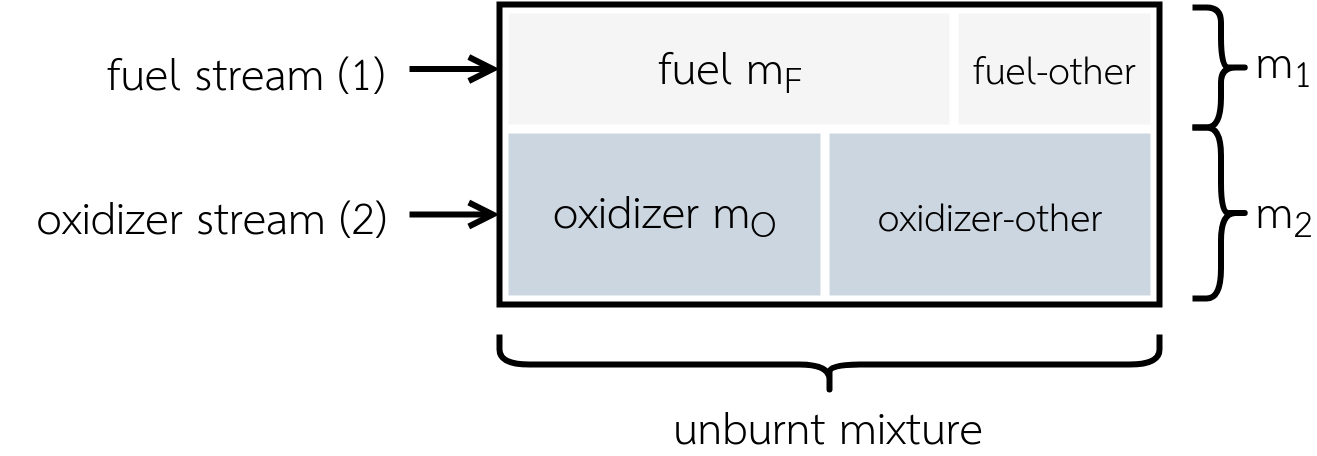
\includegraphics[width=8.5cm]{mixture-fraction.png}
\caption{Fuel-oxidizer stream system.}			
\label{fig:mixture-fraction}
\end{figure}

We may also define the mass fraction of fuel in the unburnt mixture:

\begin{equation}
Y_{u, F} = \frac{m_F}{m_{u, TOT}} = \frac{m_F}{m_1 + m_2}
\end{equation}

and mass fraction of fuel in the fuel stream:

\begin{equation}
Y_{1, F} = \frac{m_F}{m_1}
\end{equation}

These two quantities are clearly related to each other via the mixture fraction:

\begin{equation}
Y_{u, F} = \frac{m_F}{m_1 + m_2} = \frac{m_F}{m_1} \frac{m_1}{m_1 + m_2} = Y_{1, F} Z
\end{equation}

Similar reasoning can be done for the oxidizer in the oxidizer stream.

\subsection{Adiabatic flame temperature}

The adiabatic flame temperature (AdFT) is the temperature of combustion products if the combustion happens without heat exchange with the surroundings. It thus represents the maximum theoretical temperature for a given combustion system.

\subsubsection{Constant pressure AdFT}



\subsubsection{Constant volume AdFT}











\section{Energy considerations}


\subsection{Thermodynamic potentials}





\subsection{Enthalpy of formation}


\subsection{First law of thermodynamics}


\subsection{Second law of thermodynamics}



\section{Species transport}



\subsection{1-D species transport}

The mechanical transport of species can be twofold: due to a bulk motion of the fluid and/or due to molecular diffusion. Below, we consider one-dimensional binary transport.

\subsubsection{1-D diffusion from Fick's law}

One way to model molecular diffusion is to use Fick's law. It states that the mass flow rate is proportional to the concentration gradient with the constant $-\rho \mathcal{D}$:

\begin{equation}
\frac{d \dot{m}_{i, diff}}{dA} = - \rho \mathcal{D} \frac{d Y_i}{dx}
\end{equation}

In the 1-D case, the quantity $\mathcal{D}$ is called \textit{binary diffusivity} and its units are $m^2/s$. In the above equation, $\dot{m}_{i, diff}$ is the mass flux of species due to diffusion, $\rho$ is the density and $Y$ is the concentration of species.

\subsubsection{1-D bulk flow}

The bulk transport of species A is simply the fraction of the total mixture mass flux that contributes to the transport of species A. That fraction is equal to the mass fraction $Y_A$ of species A.

\begin{equation}
\frac{d \dot{m}_{i, bulk}}{dA} = Y_i \frac{d \dot{m}_{TOT}}{d A}
\end{equation}

\subsubsection{1-D binary transport}

For a one-dimensional, binary diffusion (diffusion between two species A and B) we have the mass flow rate of species A per unit area described as:

\begin{equation}
\frac{d \dot{m}_A }{dA} = Y_A \frac{d \dot{m}_{TOT}}{d A} - \rho \mathcal{D}_{AB} \frac{dY_A}{dx}
\end{equation}\label{eq:1d-bin-diff}

where $\dot{m}_{TOT} = \dot{m}_A + \dot{m}_B$.

It is worth mentioning here, that the above result does not yet contain information about possible chemical reactions in which species A and B might take part. The eq.(\ref{eq:1d-bin-diff}) describes only the pure transport of species.

\subsubsection{1-D species conservation}

Differential relations for one-dimensional species conservation can be derived by considering a 1-D control volume $\Delta x$. We now assume that the species can react, and so the mass of a particular species within the control volume can change due to transport, as well as due to creation/destruction of species in a chemical reaction. 

The change of mass of a species A in the control volume can be written as:

\begin{equation}
\frac{d m_{A, CV} }{dt} = \Big[ \frac{d \dot{m}_A}{d A} A \Big]_x - \Big[ \frac{d \dot{m}_A}{d A} A \Big]_{x + \Delta x} + r_A V
\end{equation}

where $r_A$ is the mass production rate of species A per unit volume. For further considerations we will call this term the \textit{source term}.

Substituting $m_{A, CV} = Y_A m_{CV} = Y_A \rho A \Delta x$ we get:

\begin{equation}
A \Delta x \frac{d \rho Y_{A} }{dt} = \Big[ \frac{d \dot{m}_A}{d A} A \Big]_x - \Big[ \frac{d \dot{m}_A}{d A} A \Big]_{x + \Delta x} + r_A A \Delta x
\end{equation}

Using the relation for 1-D binary diffusion from eq.(\ref{eq:1d-bin-diff}), and dividing by $A \Delta x$ we get:

\begin{equation}
\begin{aligned}
\frac{d \rho Y_{A} }{dt} = & \frac{1}{\Delta x}\Big[ Y_A \frac{d \dot{m}_{TOT}}{d A} - \rho \mathcal{D}_{AB} \frac{dY_A}{dx} \Big]_x \\
& - \frac{1}{\Delta x} \Big[ Y_A \frac{d \dot{m}_{TOT}}{d A} - \rho \mathcal{D}_{AB} \frac{dY_A}{dx} \Big]_{x + \Delta x} \\
& + r_A
\end{aligned}
\end{equation}

Finally taking the limit as $\Delta x \rightarrow 0$:

\begin{equation}
\frac{d \rho Y_{A} }{dt} = - \frac{\partial}{\partial x}\Big[ Y_A \frac{d \dot{m}_{TOT}}{d A} - \rho \mathcal{D}_{AB} \frac{dY_A}{dx} \Big] + r_A
\end{equation}






\subsection{Source terms}

\subsection{3-D species transport}

We now extend our previous relations to the 3-D case.

\subsubsection{Reaction rate considerations}


\section{Chemical kinetics}

\subsection{Reaction rate}






\section{Extension to thermal equations}




\section{Chemical reactors}








\thebibliography{}

\bibitem{Turns} S. R. Turns, \textit{An Introduction to Combustion: Concepts and Applications}, Second Edition, 2000 \label{bib:turns}

\bibitem{Pitsch} H. Pitsch, \textit{Combustion Theory and Applications in CFD}, Lecture Series \label{bib:pitsch}


 \label{bib:pope}


\end{document}
